\chapter{Chapter 2. Data sets and pre-processing}\label{ch:ch2_data}

The data in this study are time series measurements from the Time History of Events and Macroscale Interactions during Substorms-Acceleration, Reconnection, Turbulence and Electrodynamics of the Moon’s Interaction with the Sun (THEMIS-ARTEMIS) mission and the Magnetospheric Multiscale (MMS) mission. The former mission seeks to investigate substorms in the Earth's magnetosphere, observe the Earth's radiation belts, and examine solar wind-magnetosphere interaction on the day-side. 


\section{THEMIS data set}
The THEMIS spacecraft are optimized for observing different regions of the magnetosphere and near-Earth solar wind. The five THEMIS probes (THM A-E) are traversing near-Earth space in different regions and orbits according to the science phases. THEMIS-B and THEMIS-C were reassigned as ARTEMIS-P1 and ARTEMIS-P2, respectively, in 2009 to facilitate observations at lunar Lagrange points 1 and 2. The separation between the probes, specifically during the mission phases in which simultaneous observation between the solar wind and magnetosheath are available, makes this mission ideal for use in this study.

Aboard each of the five THEMIS probes, identical Electrostatic Analyzer (ESA) instruments measure ion and electron distribution functions in three dimensions via spherical top-hat electrostatic analyzers \citep{McFadden:2008}. The observable range of energy fluxes of the ESA instrument is approximately 1.6-25 keV for ions and 2-32 keV for electrons. The Fluxgate Magnetometers (FGM) on each THEMIS probe \citep{Auster:2008} are single digital fluxgate magnetometers with a sensor at the end of a 2 meter boom. Because of the mission goals related to magnetic reconnection during substorms, the fluxgate magnetometers are very sensitive, with precision down to 0.1 nT, and operate in the range of 0.1-25000 nT \citep{Auster:2008}. Figure \ref{fig:thm-diagram} displays the arrangement of the instruments on a singular THEMIS probe. The FGM is located on the end of the boom, with the ESA and other instruments placed around the body of the spacecraft.

\begin{figure}
    \centering
    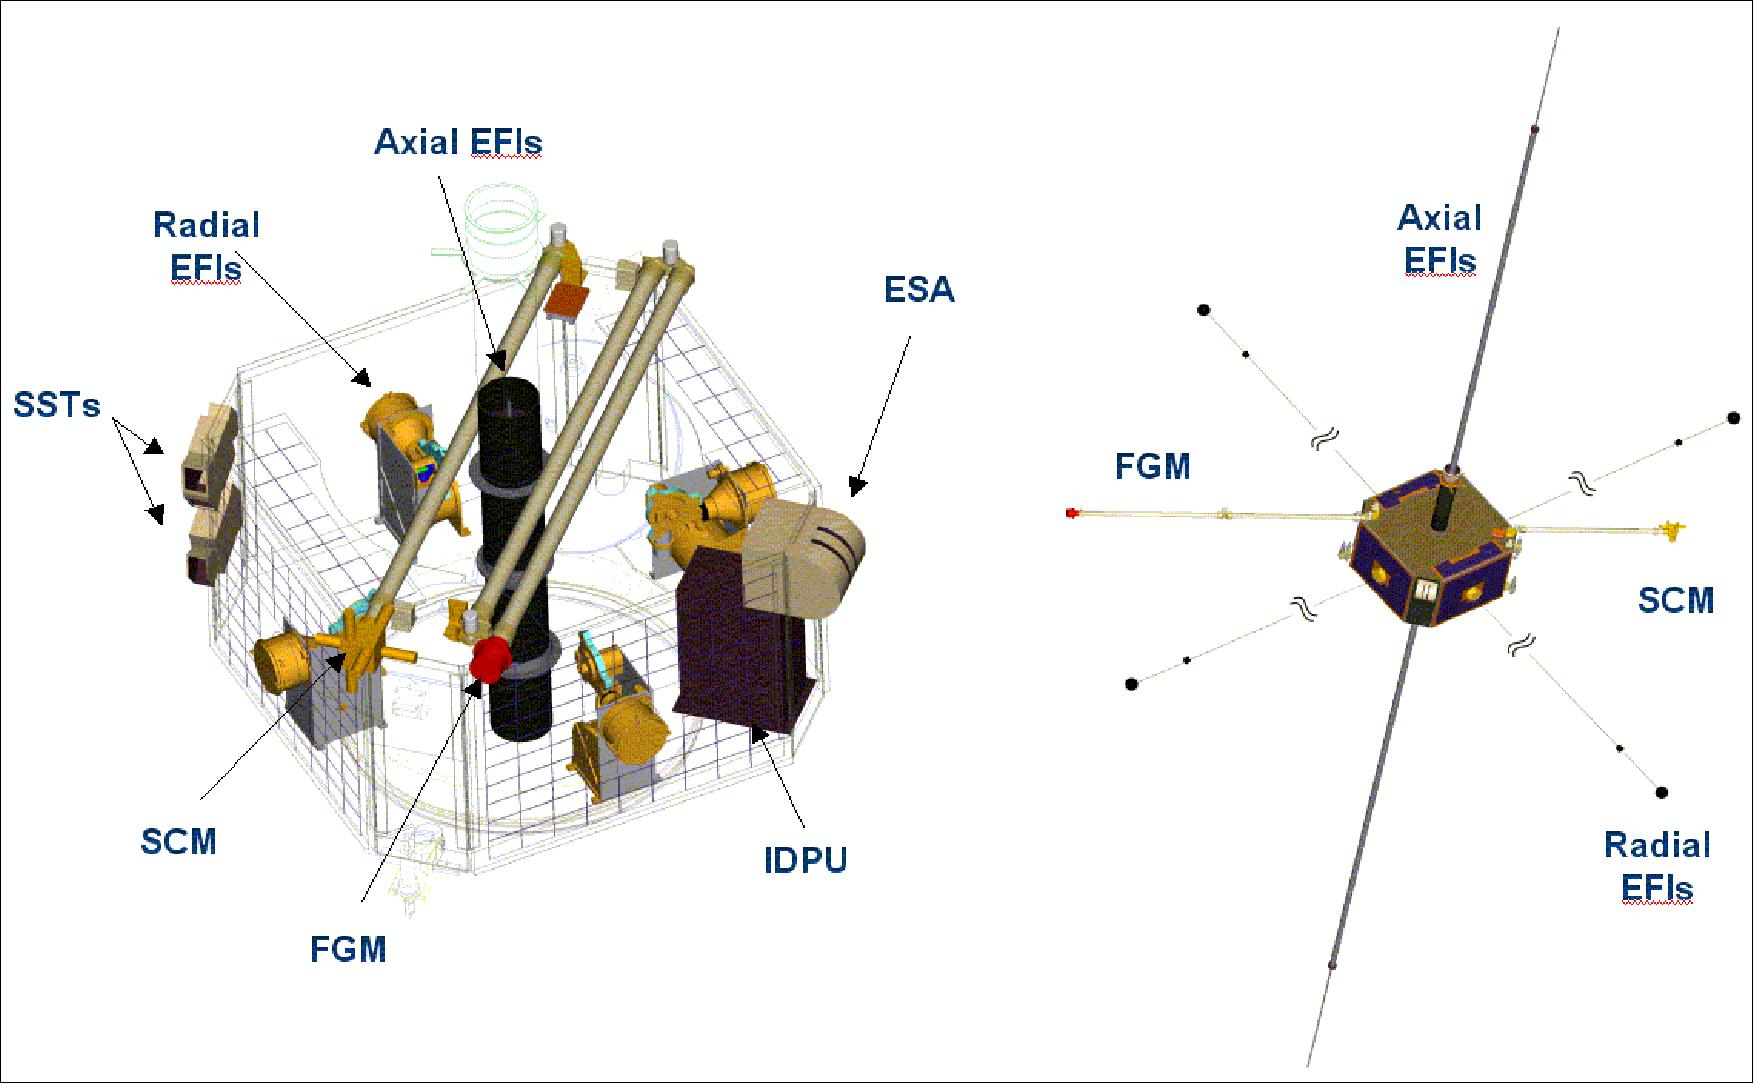
\includegraphics[width=\textwidth]{Figures/Instrumentation/THM_diagram.jpeg}
    \caption[Configuration of instruments on a singular THEMIS probe]{Configuration of instruments on a singular THEMIS probe. On the left, all of the instruments are shown, including the FGM and ESA. On the right, the Fluxgate Magnetometer (FGM) can be seen at the end of its 2 meter long boom, along with the Search Coil magnetomter (SCM) and Electric Field Instrument (EFI) \citep{eoPortal}.}
    \label{fig:thm-diagram}
\end{figure}

\section{MMS dataset}
The MMS mission, comprised of four identical probes in a tetrahedral formation, also moves through the solar wind and magnetosheath. The magnetic field data from MMS come from the Fluxgate Magnetometer (FGM), which is part of the FIELDS suite on MMS \citep{Torbert:2016}. The MMS FIELDS suite is responsible for measuring the magnetic and electric fields. The FGM is comprised of two magnetometers on each spacecraft, one analog (AFG) and one digital (DFG). The magnetometers measure the magnetic field components with three-axis sensors \citep{Torbert:2016}. The two magnetometers are located on opposite sides of the spacecraft, each at the end of a five meter long boom (see Figure \ref{fig:fgm-mms}). Because there are two magnetometers on each spacecraft, they provide redundant data which is used to cross-calibrate the AFG and DFG instruments \citep{Torbert:2016}. The other instruments of the FIELDS suite are the Search Coil Magnetometer (SCM), which measures the magnetic field fluctuations over 1 Hz-6 kHz. The Spin-plane Double-Probes (SDP) and the Axial Double Probe (ADP) measure the electric field in the spin plane and along the spin axis, respectively. The Electron Drift Instrument measures ambient electron flux, and the EDI is used to conduct geometric measurements of the electric field and time-of-flight measurements for the magnetic field.
% determination of the offsets in the spin axis component of the AFG and DFG

\begin{figure}
    \centering
    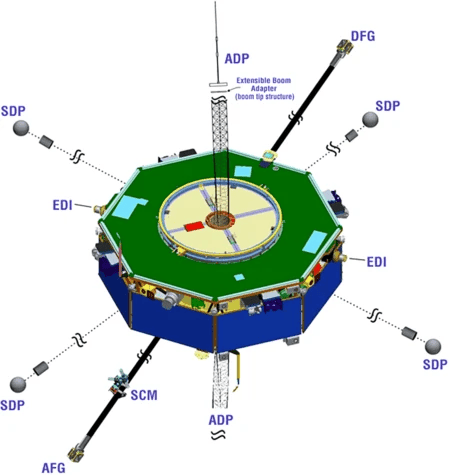
\includegraphics[width=0.7\textwidth]{Figures/Instrumentation/Torbert_Figure7.png}
    \caption[MMS FIELDS suite]{The MMS FIELDS suite on an individual probe, which measures magnetic and electric fields. The analog fluxgate magnetometer (AFG) and digital fluxgate magnetometer (DFG) are located at the ends of the two five meter booms, in the bottom left corner and top right corner. The Search Coil Magnetometer (SCM),  Electron Drift Instrument (EDI), Spin-plane Double-Probes (SDP), and the Axial Double-Probes (ADP) complete the FIELDS suite aboard each MMS spacecraft \citep{Burch:2024}.}
    \label{fig:fgm-mms}
\end{figure}

The Fast Plasma Investigation (FPI) \citep{Pollock:2016} instrument on MMS measures the velocity-space distribution of ions and electrons in the plasma in near-Earth space, from which their energy and velocity can be ascertained. Four dual electron spectrometers (DES) and four dual ion spectrometers (DIS) are evenly placed around each of the four probes, which are then connected to individual (IDPU) and central (CDPU) data processing units \citep{Pollock:2016}. The spectrometers measure the energy of the ions and electrons from 10 eV to 30 keV by measuring their differential directional flux distributions at a time resolution of 150 ms (for ions) and 30 ms (for electrons). Figure \ref{fig:fpi-mms} displays the layout of the FPI spectrometers aboard each MMS spacecraft.

% \begin{figure}
%     \centering
%     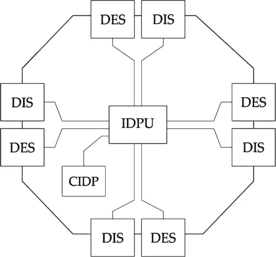
\includegraphics[width=0.7\textwidth]{Figures//Instrumentation/Torbert_Figure4.png}
%     \caption[Schematic of DIS and DES instruments aboard MMS]{Schematic of the ion (DIS) and electron (DES) spectrometers, which shows how the instruments are connected to the individual instrument data processing unit (IDPU), which in turn is connected to the central data processing unit (CDPU) \citep{Pollock:2016}.} 
%     \label{fig:fpi-mms-schematic}
% \end{figure}

\begin{figure}
    \centering
    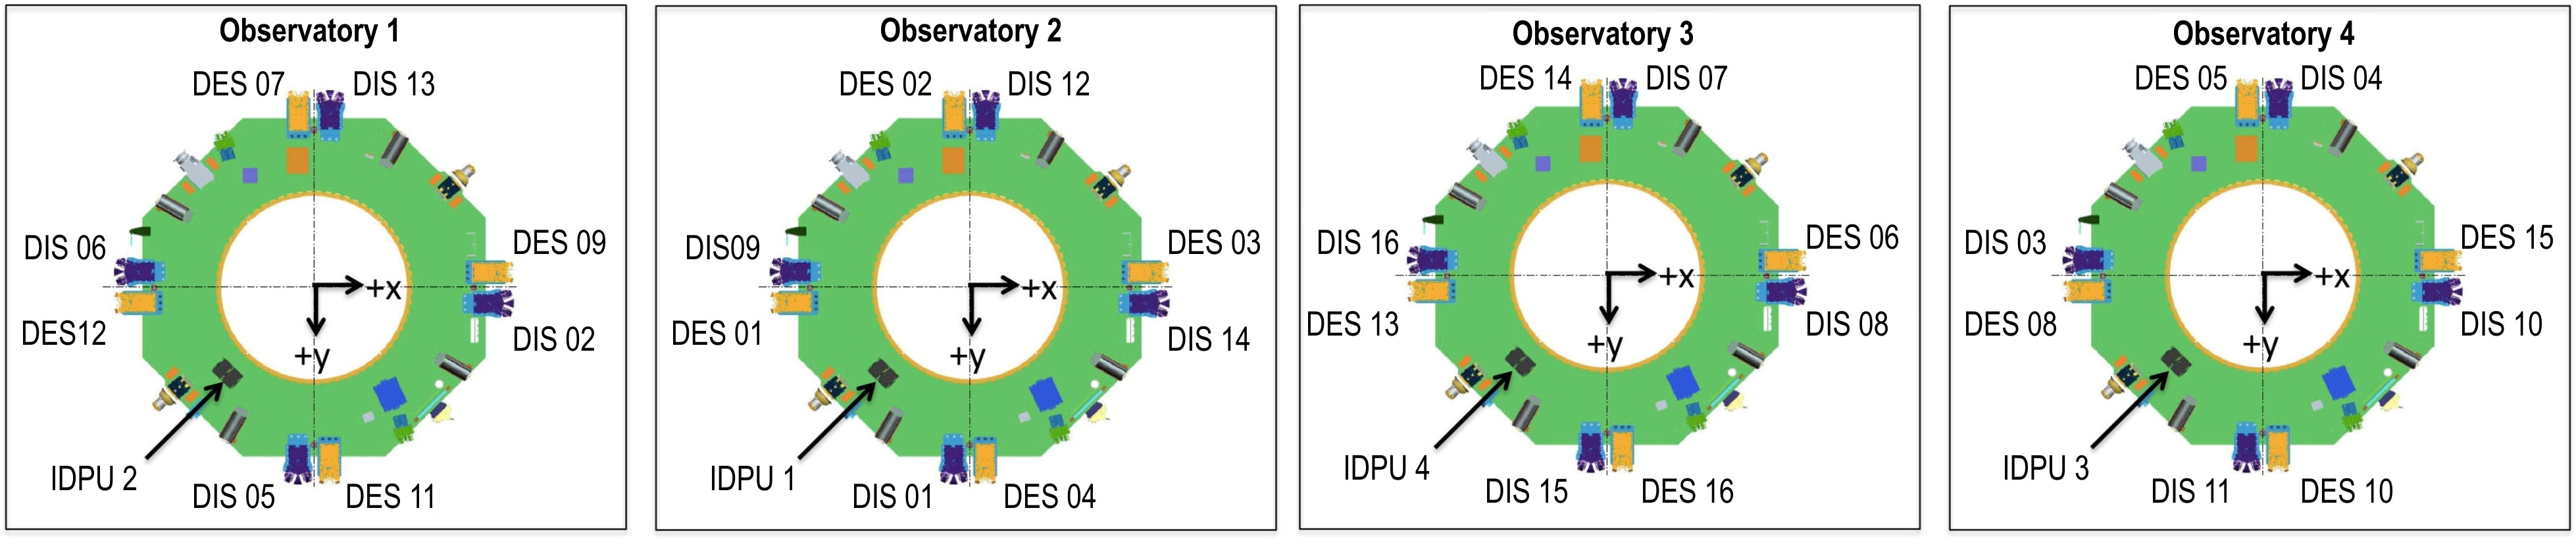
\includegraphics[width=\textwidth]{Figures//Instrumentation/Pollock_Figure5.jpg}
    \caption[MMS FPI instrument suite]{Diagram showing the full FPI instrument suite across each of the MMS spacecraft \citep{Pollock:2016}.}
    \label{fig:fpi-mms}
\end{figure}

\begin{figure}
    \centering
    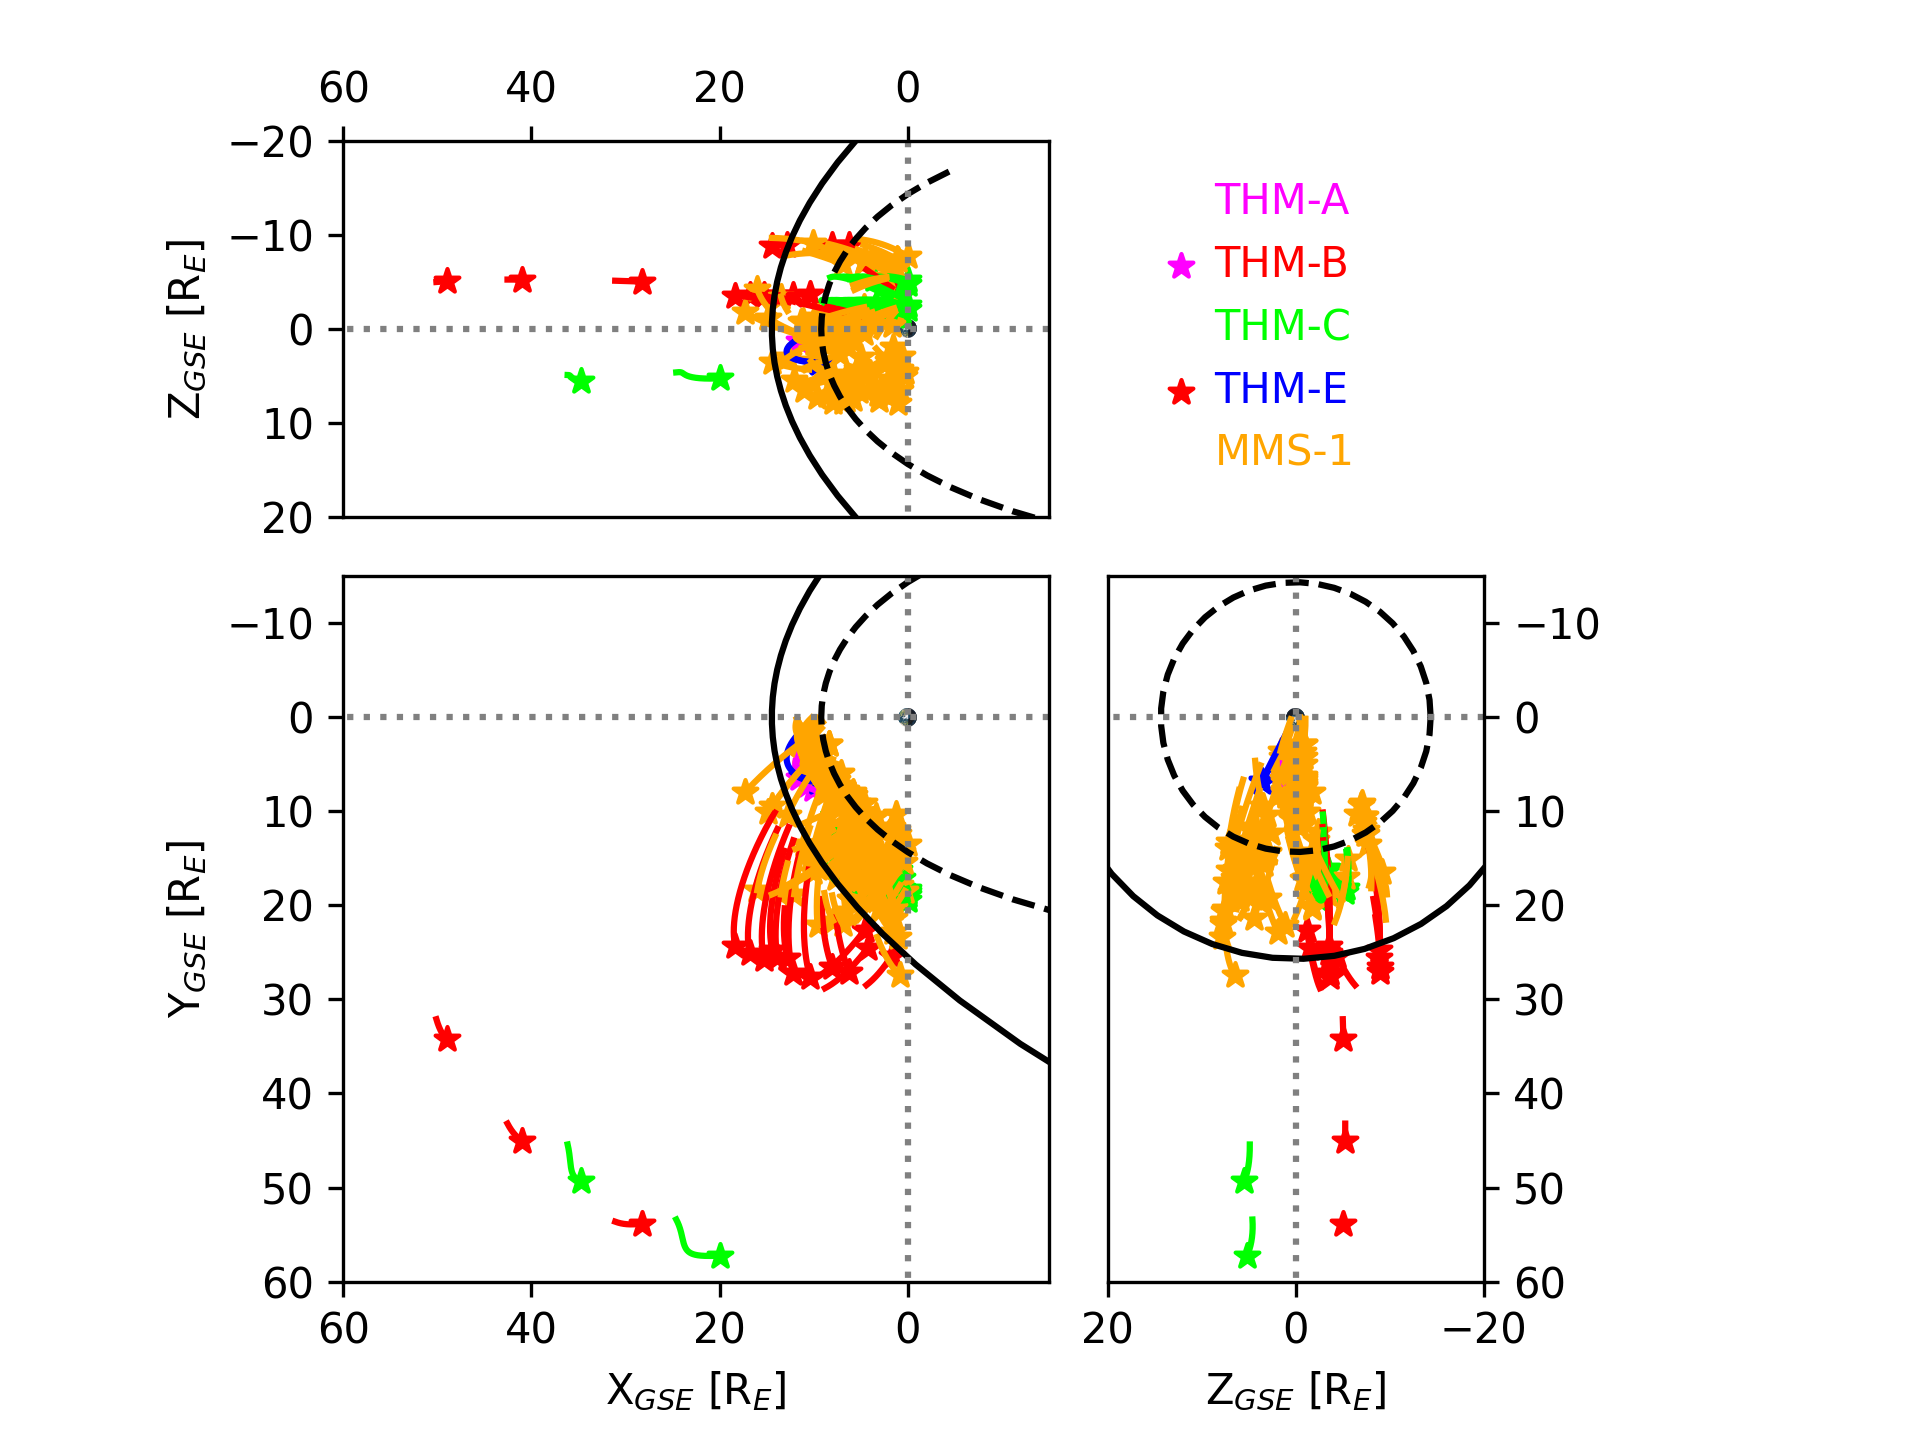
\includegraphics[width=\textwidth]{Figures/Orbits/all_TE_orbits_xy_xz_yz.png}
    \caption[Orbits for all observation periods]{Orbits for all analysis time periods are shown in the Geocentric Solar Ecliptic (GSE) coordinates for THEMIS probes A, B, C, and E (THM-A, THM-B, THM-C, THM-E) and MMS-1 probe (see legend), with the stars marking the end of each orbit period. The approximate nominal locations of the magnetopause (dashed black line) modeled using the \cite{Shue:1997} model and bow shock (solid black line) modeled using \cite{SlavinHolzer:1984} are shown, based on the IMF data obtained for one period in 2015 only.}
    \label{fig:all-orbits-plot}
\end{figure}

\section{Selection and pre-processing}
Hours-long periods of THEMIS data with cadence $\Delta t\sim$3 seconds and MMS data with $\Delta t=4.5$ seconds in the magnetosheath and near-Earth solar wind are chosen such that each analysis interval is entirely contained in one region to avoid transition regions. Figure \ref{fig:all-orbits-plot} shows the orbit segments of the THEMIS and MMS-1 probes for the selected time periods. The orange orbit lines display portions of the MMS-1 orbits from 2015-2023. The pink, red, green, and blue orbit lines show the THEMIS orbits in 2008, 2009, 2018, and 2022. The solid curve and dashed curve are the estimated bow shock and magnetopause boundaries \citep{SlavinHolzer:1984,Shue:1997}. These time periods, ranging in lengths from approximately 6 hours to 26 hours, are identified by looking at time series data and finding data segments bounded by simultaneous changes in magnetic field, plasma density, velocity, and ion spectra. Short instances of possible bow shock crossings (including multiple crossings) are identified in certain time periods, and the events identified in these crossing periods are removed from the final lists.

Figures \ref{fig:timeseries-MMS-magnetosheath} and \ref{fig:timeseries-THM-magnetosheath} are examples of two observed time periods in the magnetosheath from MMS-1 and THM-C, respectively. Both figures show the time series of magnetic field, plasma velocity, proton density, temperature, and ion energy spectra, as well as calculated values such as Alfv\'en velocity and proton beta. These quantities are used in our analysis, and also to identify the region in which the spacecraft was located. During the 19-20 June 2009 time period, THM-C experienced a bow shock crossing, which is denoted by the grey-shaded interval in Figure \ref{fig:timeseries-THM-magnetosheath}. By looking at the time series data during the whole period, and identifying changes in the data such as magnetic field and ion spectra that were consistent with bow shock crossings \citep{Lalti:2022,Trotta:2022}, periods where the spacecraft were experiencing a bow shock crossing were identified. The events in the bow shock crossing periods are removed from the final event list.

\begin{figure}
    \centering
    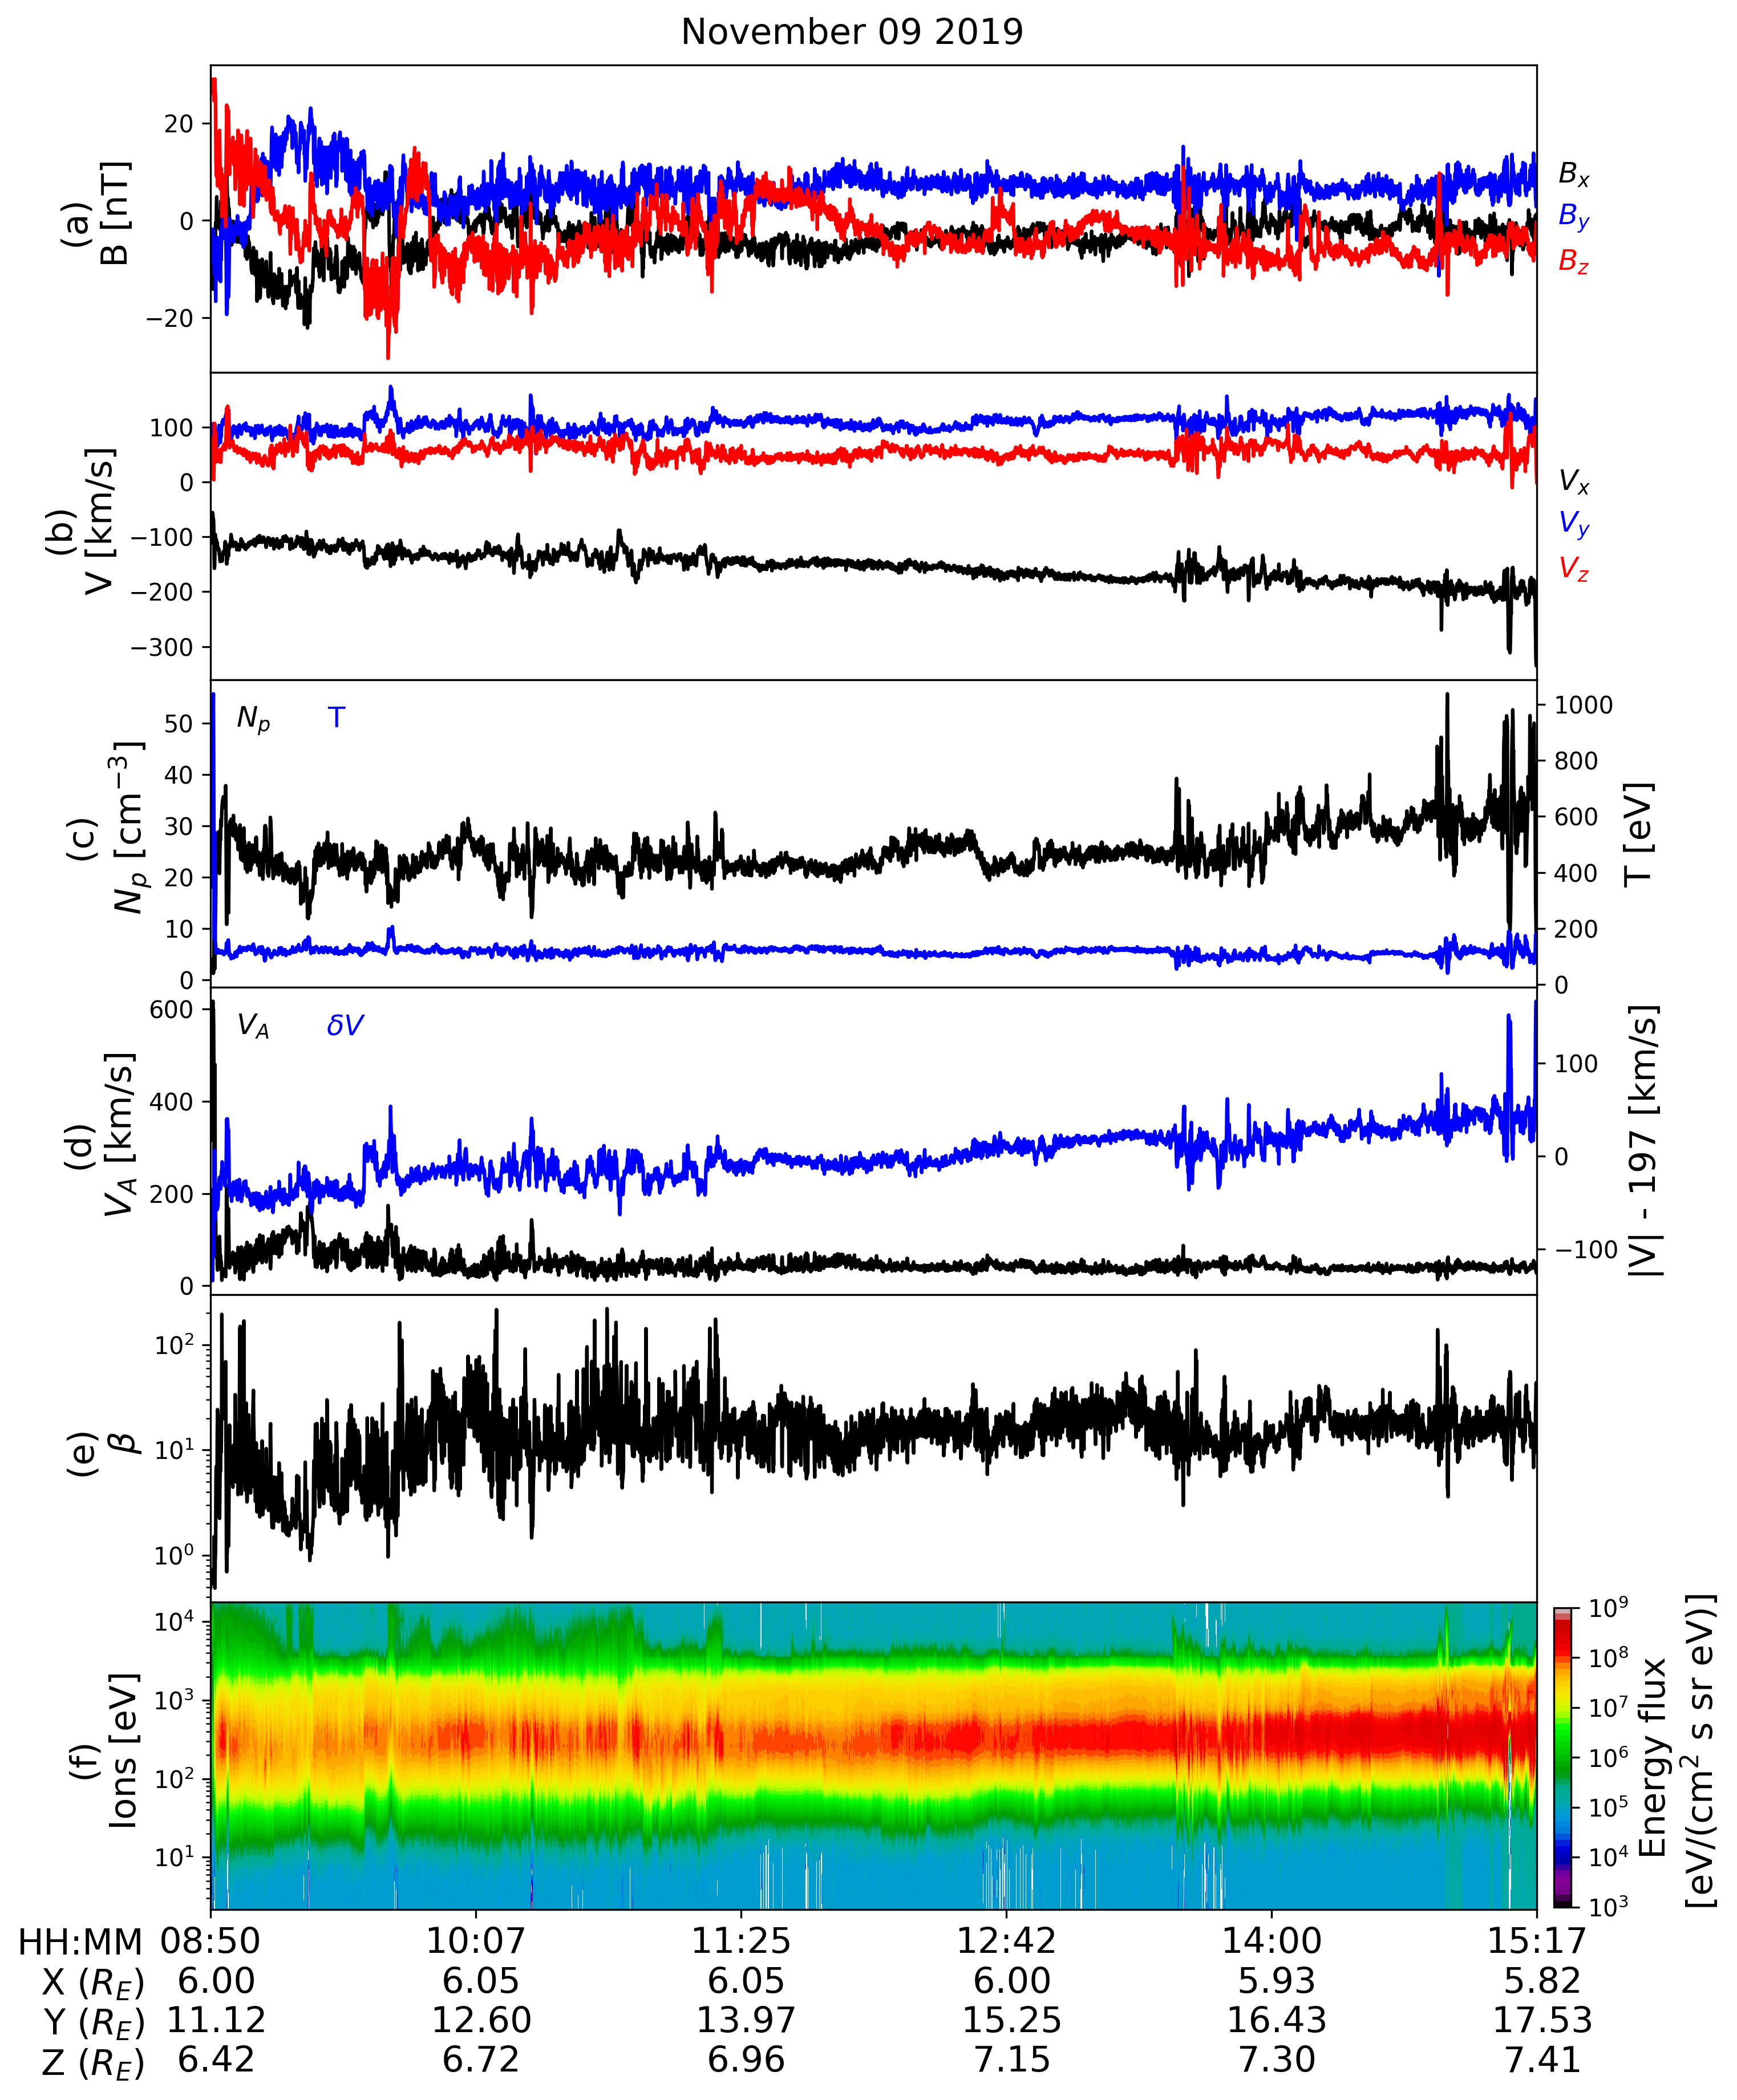
\includegraphics[width=0.9\textwidth]{Figures/Time series/timeseries_09112019_MMS1.png}
    \caption[Time series data observed in the magnetosheath on 9 November 2019]{Time series data observed by MMS-1 for $\sim$6 hours in the magnetosheath on 9 November 2019, with supplementary ephemeris data in GSE coordinates. The panels show a) magnetic field components, b) the components of flow velocity $\mathbf{V_{sw}}$, c) proton density and temperature, d) Alfv\'en speed and fluctuations of the magnitude of the velocity, e) proton beta, and f) ion spectra.}
    \label{fig:timeseries-MMS-magnetosheath}
\end{figure}

\begin{figure}
    \centering
    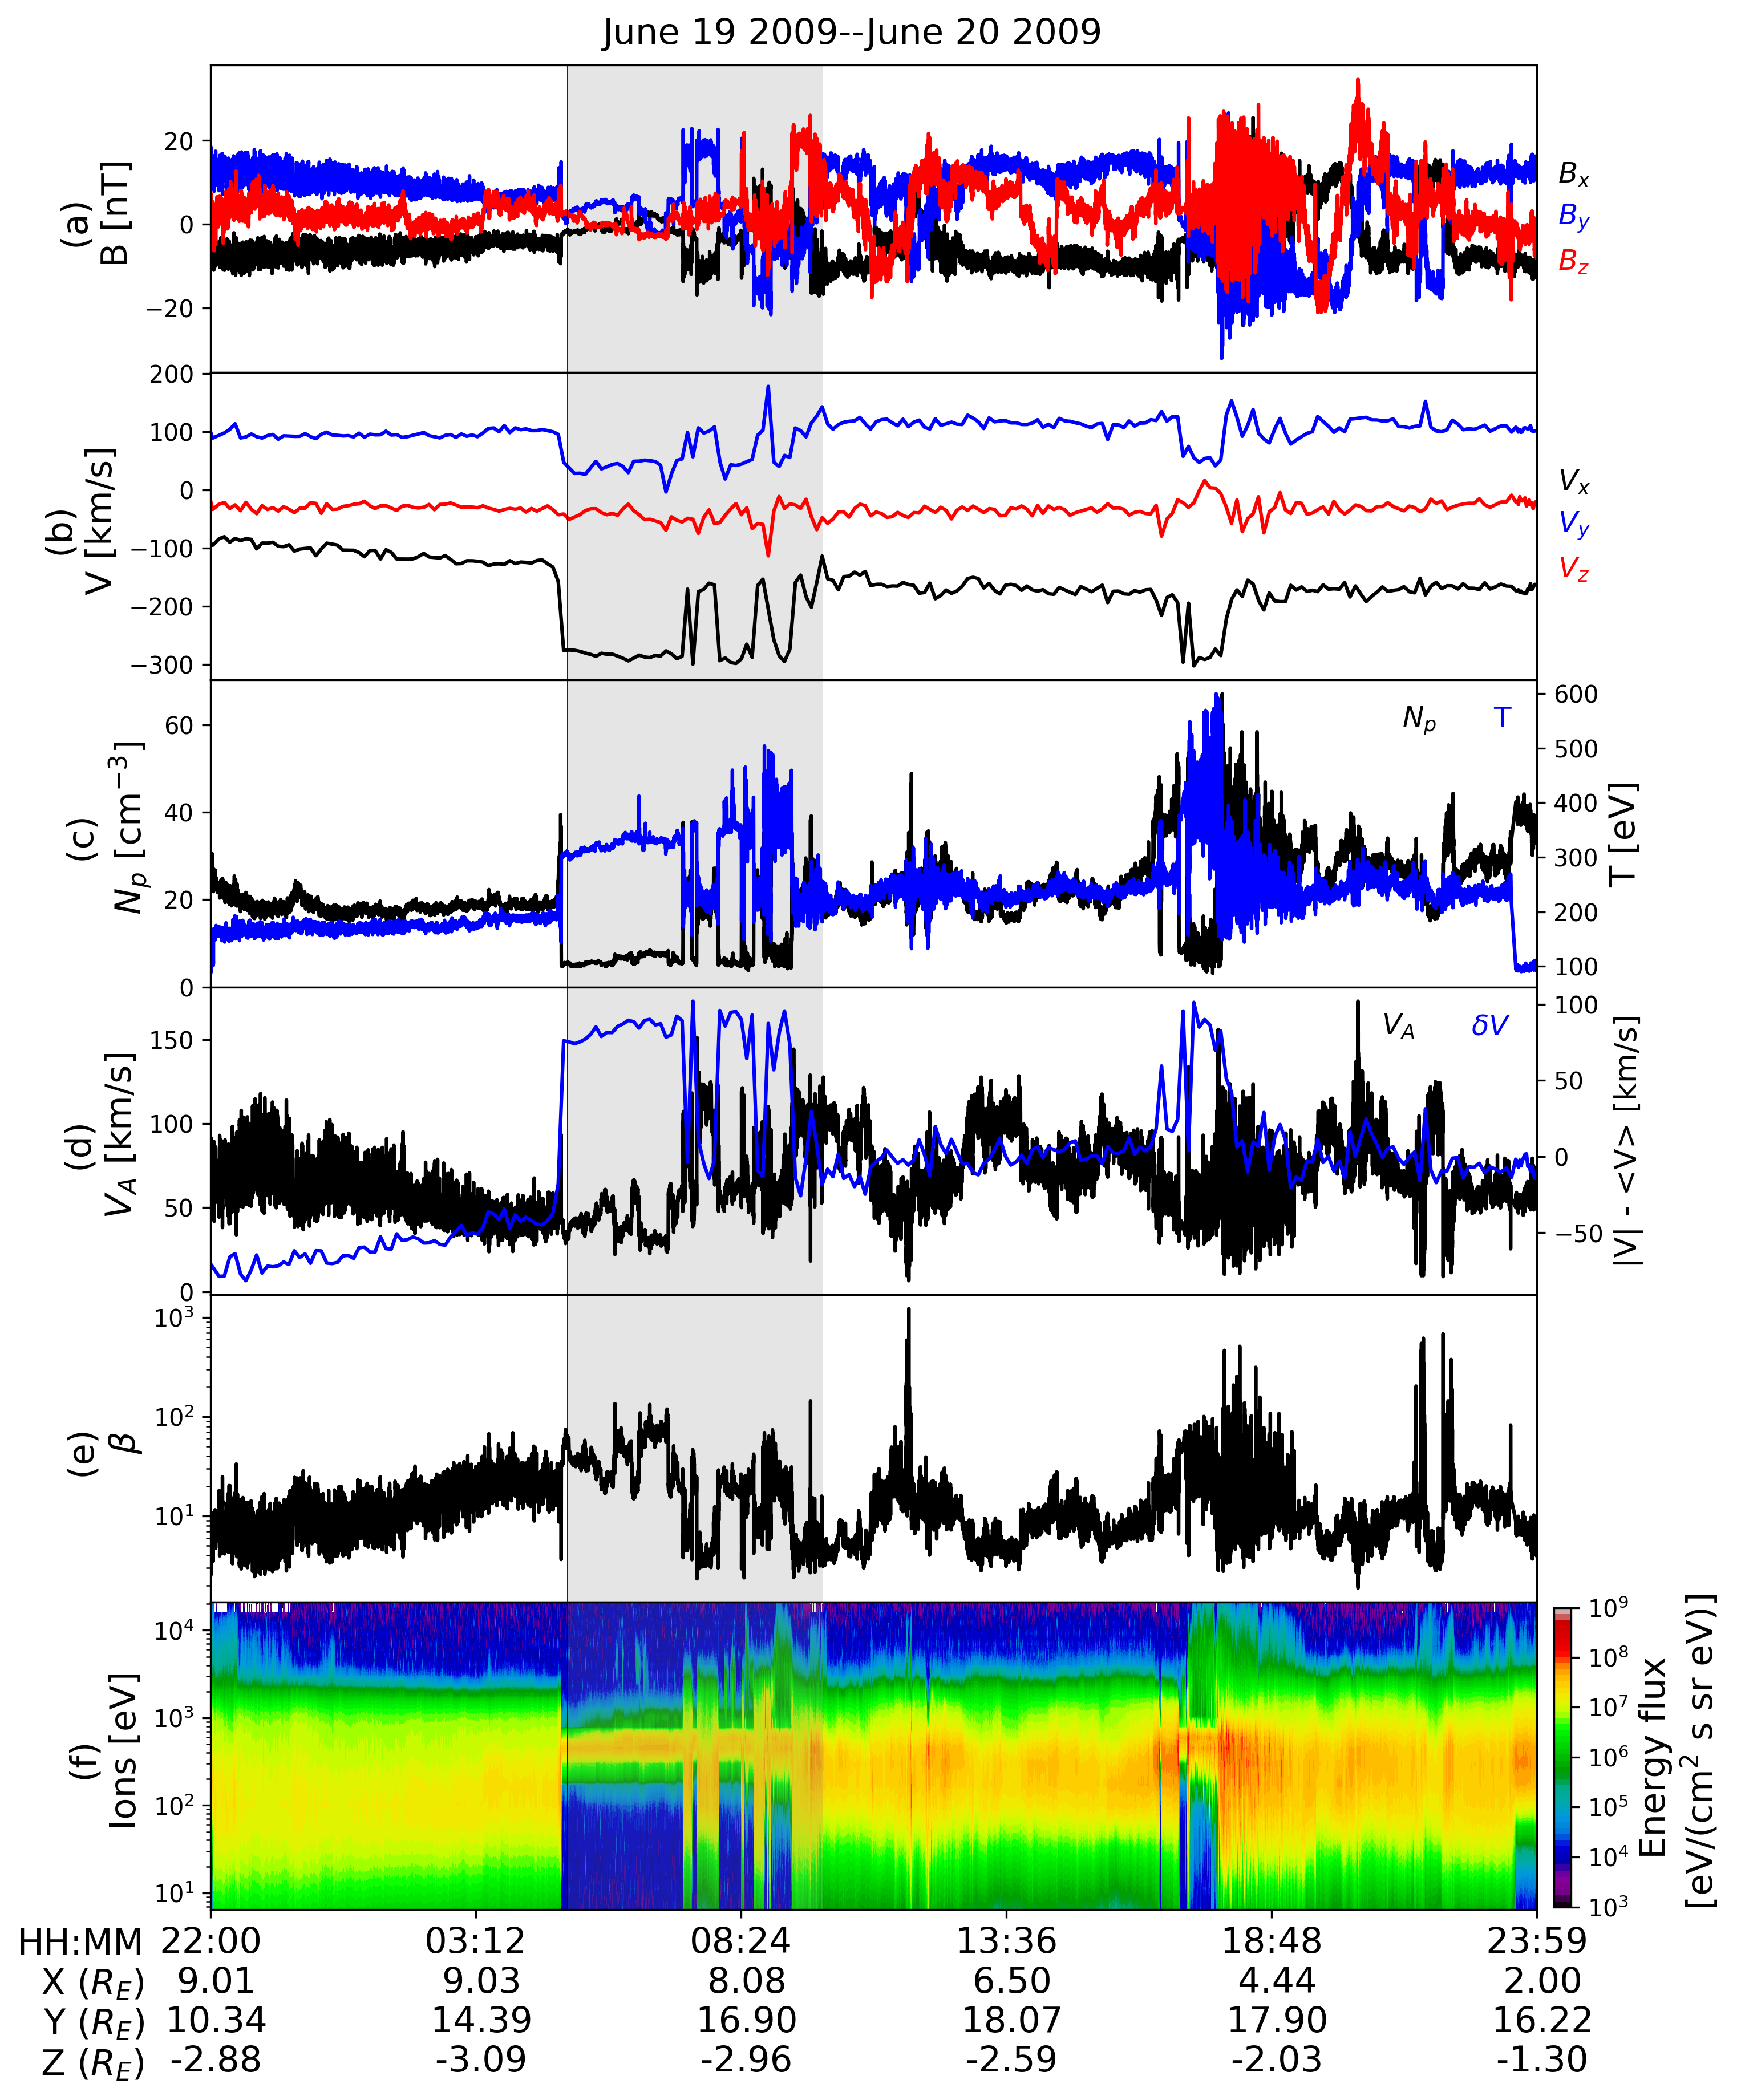
\includegraphics[width=0.9\textwidth]{Figures/Time series/timeseries_19062009_THMC.png}
    \caption[Time series data observed in the magnetosheath during 19-20 June 2009]{Time series data observed on 19-20 June 2009 by THM-C. This observation period spans $\sim$26 hours in the magnetosheath, with a bow shock crossing (grey region) identified during 5:00-10:00 UT on 20 June 2009. Similar to Figure \ref{fig:timeseries-MMS-magnetosheath}, the panels show the a) magnetic field, b) velocity, c) proton density and temperature, d) Alfv\'en speed and fluctuations of the magnitude of the velocity, e) proton beta, and f) ion spectra.}
    \label{fig:timeseries-THM-magnetosheath}
\end{figure}

% Toy-Edens list
In addition to manually identifying periods in the solar wind and the magnetosheath, the published list of MMS data periods in the magnetosheath and solar wind from \cite{ToyEdens:2024} was also used. Their work focused on using unsupervised clustering to classify plasma regions in 8 years' worth of dayside MMS data \citep{ToyEdens2:2024}. The 1-minute resolution data was classified into the following regions: solar wind, ion foreshock, magnetosheath, and magnetosphere. The \cite{ToyEdens:2024} list contains over 9000 time periods in which MMS-1 to MMS-4 probes were identified to be solidly in the magnetosheath, with the minimum period being 15 minutes in length. The list of \cite{ToyEdens:2024} was refined by taking time periods with a duration longer than 5 hours for both the solar wind and magnetosheath regions, which is comparable to the shortest identified time period of THEMIS data. After further refining their magnetosheath list to the region downstream of the quasi-perpendicular bow shock (corresponding to a condition that the spacecraft location of $Y_{GSE}>0$), one-hundred and seven time periods were obtained to be used in this study. Fifty-eight periods, in which MMS traversed the solar wind upstream of the quasi-perpendicular bow shock, were obtained from the \cite{ToyEdens:2024} solar wind list. \cite{ToyEdens2:2024} include all MMS probes in their analysis; however, I only consider MMS-1 since presumably the other 3 MMS probes are in the same region and I only report the results from MMS-1. In total, from the \cite{ToyEdens:2024} list and from our own identification, there were 130 time periods of data identified in the magnetosheath from THM-A, THM-C, THM-E, and MMS-1; and 77 periods identified in the solar wind from THM-B, THM-C, and MMS-1. The total lengths of the search time periods for our study are 1051 hours in the magnetosheath and 676 hours in the solar wind. A summary table of the observation search intervals can be found in Appendix \ref{appendix:observation-periods}. Table \ref{tab:data-products} displays the data products used in this work.

\begin{table}
    \centering
    \begin{tabular}{lcccc}
\hline
Data product            & Instrument & Symbol           & Units        & Cadence [s] \\
\hline
Magnetic field vector 	& FGM      & $B_X, B_Y, B_Z$  & nT                     & 2.74 - 4.295 \\
Flow velocity vector  	& ESA       & $V_X, V_Y, V_Z$  & km/s                  & 2.74 - 360$^a$ \\
Proton number density	& ESA       & $N_p$            	& cm$^{-3}$            & 2.74 - 4.295 \\
Proton temperature    	& ESA       & $T$            	& eV                   & 2.74 - 4.295 \\
Ion energy spectra    	& ESA       &                  	& eV/(cm$^2$ s sr eV)  & 2.74 - 4.295 \\
\hline
Magnetic field vector 	& FGM      & $B_X, B_Y, B_Z$  & nT                    & 4.5 \\
Flow velocity vector  	& FPI      & $V_X, V_Y, V_Z$  & km/s                  & 4.5 \\
Proton number density 	& FPI      & $N_p$            & cm$^{-3}$             & 4.5 \\
Proton temperature    	& FPI      & $T$              & eV                    & 4.5 \\
Ion energy spectra   	& FPI      &                  & eV/(cm$^2$ s sr eV)   & 4.5 \\
\hline
\end{tabular}
    \caption[Data products from THEMIS and MMS]{Data products from THEMIS (top) and MMS (bottom) used in this study. For the flow velocity vector from THEMIS, there are some periods in which 6-minute data was up-sampled to match the $\sim$ 3-second data.}
    \label{tab:data-products}
\end{table}

%A significant portion (green and red lines) of the coordinated analysis data periods are hidden behind the orange MMS orbit lines; however, the orbit plots for the coordinated analysis periods can be found in the appendix.

% note: 107 periods were used for detection; however of the total events, 5 events overlapped with mine that I had already run and then there was 1 period with data not available and 3 with time periods not really inside the magnetosheath by visual identification of time series data

\section*{Open Research}
The MMS and THEMIS data \citep{Torbert:2016,Pollock:2016} used in this study was retrieved from the NASA Science Data Center via the PySPEDAS software, which is open source and publicly available at \url{https://github.com/spedas/pyspedas} under an MIT license. The \cite{ToyEdens:2024} database of MMS periods in the solar wind and magnetosheath is available open access at \url{https://zenodo.org/records/11032322}, and the algorithm to generate this data is described in \cite{ToyEdens2:2024}.